% !TeX root = ../main.tex
\section{Virtual machines}
\label{sec:vm}

A tree-walking interpreter dispatches on every node each time it runs; a
native compiler needs instruction selection, register allocation and a back
end per machine. A bytecode \textbf{virtual machine} sits between the two: the
AST is compiled once into the instructions of an abstract machine, and a
simple interpreter runs those instructions. The abstract machine of SIMP in
the semantics notes, with its control stack and its result stack, is a
machine of this kind. This section follows Nystrom~\cite[Part~III]{nystrom2021crafting}.

\subsection{Stack machines and register machines}

A \textbf{stack machine} (the JVM, the CPython virtual machine) keeps a stack of
operands: each instruction takes its operands from the top of the stack and
pushes its result. A \textbf{register machine} (the virtual machine of Lua
since version 5) has virtual registers, and each instruction names its
operands and its destination, as machine code does. For \texttt{(a + b) * c}:
\begin{center}
\begin{minipage}[t]{0.35\textwidth}
\begin{lstlisting}
push a
push b
add
push c
mul
\end{lstlisting}
\end{minipage}
\hspace{1cm}
\begin{minipage}[t]{0.4\textwidth}
\begin{lstlisting}
add r0, a, b
mul r1, r0, c
\end{lstlisting}
\end{minipage}
\end{center}
The stack version has five simple instructions, and its compiler only walks
the AST in postorder, emitting the operands before the operator. The register
version has two instructions, but its compiler has to decide which register
holds each value, a version of the register allocation problem of
Section~\ref{sec:ir}. The stack machine moves more data on and off the stack;
the register machine needs a more complex compiler.

\subsection{The dispatch loop}

The core of the virtual machine is a \textbf{dispatch loop}: fetch the next
instruction, select the code for it, run it, repeat.
\coderange{C}{c/vm.c}{run}
The \texttt{switch} is usually compiled to a jump table, like the one of
Section~\ref{sec:representation}, and every instruction goes back to the top
of the loop. Faster virtual machines replace the central \texttt{switch} by
\emph{threaded code}: each handler ends with a jump to the handler of the next
instruction, taken from a table, without going back through the loop. In C
this needs an extension of GCC and Clang (labels as values), so portable
virtual machines keep the \texttt{switch}.

\subsection{A trace}

The program \texttt{print (2 + 3) * 4} compiles to
\coderange{C}{c/vm.c}{program}
where each \texttt{OP\_CONSTANT} is followed by an index into the table of
constants. Table~\ref{tab:vm-trace} shows the stack after each instruction,
and Figure~\ref{fig:vm-stack} the same stack drawn at each step. Each row is
one iteration of the loop.

\begin{table}[h]
\centering
\begin{tabular}{@{}lll@{}}
\toprule
Instruction & Effect & Stack after \\
\midrule
\texttt{CONSTANT 2} & push 2 & $[2]$ \\
\texttt{CONSTANT 3} & push 3 & $[2, 3]$ \\
\texttt{ADD} & pop 3 and 2, push $2 + 3$ & $[5]$ \\
\texttt{CONSTANT 4} & push 4 & $[5, 4]$ \\
\texttt{MULTIPLY} & pop 4 and 5, push $5 \times 4$ & $[20]$ \\
\texttt{PRINT} & pop 20 and print it & $[\,]$ \\
\bottomrule
\end{tabular}
\caption{Trace of \texttt{print (2 + 3) * 4}.}
\label{tab:vm-trace}
\end{table}

\begin{figure}[h]
\centering
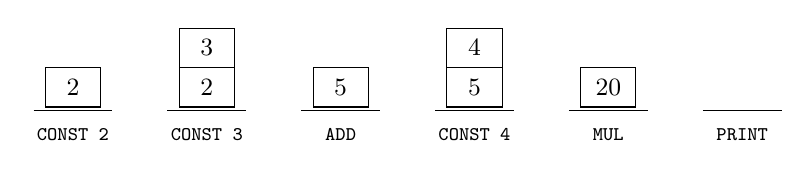
\begin{tikzpicture}[c/.style={draw, minimum width=7mm, minimum height=5mm, font=\small}]
  \foreach \x/\lbl/\vals in {0/{CONST 2}/{2}, 1.7/{CONST 3}/{2,3}, 3.4/{ADD}/{5}, 5.1/{CONST 4}/{5,4}, 6.8/{MUL}/{20}} {
    \foreach \v [count=\i] in \vals {
      \node[c] at (\x, 0.5*\i) {\v};
    }
    \draw (\x-0.5,0.2) -- (\x+0.5,0.2);
    \node[font=\scriptsize\ttfamily] at (\x,-0.1) {\lbl};
  }
  \draw (8.0,0.2) -- (9.0,0.2);
  \node[font=\scriptsize\ttfamily] at (8.5,-0.1) {PRINT};
\end{tikzpicture}
\caption{The operand stack after each instruction; the top is drawn highest.}
\label{fig:vm-stack}
\end{figure}

\subsection{Exercises}

\begin{exercise}
Compile \texttt{(a - b) * (c + d)} for the stack machine and for the register
machine.
\end{exercise}

\paragraph{Solution.} Stack machine: \texttt{push a}, \texttt{push b},
\texttt{sub}, \texttt{push c}, \texttt{push d}, \texttt{add}, \texttt{mul}, seven
instructions, with at most three values on the stack. Register machine:
\texttt{sub r0, a, b}, \texttt{add r1, c, d}, \texttt{mul r2, r0, r1}, three
instructions and three registers (two if \texttt{r2} reuses \texttt{r0}).

\begin{exercise}
Trace \texttt{CONSTANT 10}, \texttt{CONSTANT 4}, \texttt{SUBTRACT},
\texttt{CONSTANT 2}, \texttt{MULTIPLY}, \texttt{PRINT}.
\end{exercise}

\paragraph{Solution.} The stack goes through $[10]$, $[10, 4]$, $[6]$, $[6, 2]$,
$[12]$, $[\,]$, and 12 is printed. The second test of \texttt{vm.c} runs this
program.

\begin{exercise}
Why can the compiler for the stack machine work with a postorder walk of the
AST?
\end{exercise}

\paragraph{Solution.} In postorder the code of the operands comes before the
code of the operator. When the operator runs, its operands are the values on
top of the stack, in order, and its result takes their place. The compiler
never has to name where a value is.
